\documentclass[crop,tikz]{standalone}

\usepackage[utf8]{inputenc}

% 'crop' is the default for v1.0, before it was 'preview'
%\usetikzlibrary{...}% tikz package already loaded by 'tikz' option

%tikz structures and patterns
\usetikzlibrary{patterns}

%this defines a fill pattern called hexagons
\def\hexagonsize{0.4cm}
\pgfdeclarepatternformonly
  {hexagons}% name
  {\pgfpointorigin}% lower left
  {\pgfpoint{3*\hexagonsize}{0.866025*2*\hexagonsize}}%  upper right
  {\pgfpoint{3*\hexagonsize}{0.866025*2*\hexagonsize}}%  tile size
  {% shape description
   \pgfsetlinewidth{1.2pt}
   \pgftransformshift{\pgfpoint{0mm}{0.866025*\hexagonsize}}
   \pgfpathmoveto{\pgfpoint{0mm}{0mm}}
   \pgfpathlineto{\pgfpoint{0.5*\hexagonsize}{0mm}}
   \pgfpathlineto{\pgfpoint{\hexagonsize}{-0.866025*\hexagonsize}}
   \pgfpathlineto{\pgfpoint{2*\hexagonsize}{-0.866025*\hexagonsize}}
   \pgfpathlineto{\pgfpoint{2.5*\hexagonsize}{0mm}}
   \pgfpathlineto{\pgfpoint{3*\hexagonsize+0.2mm}{0mm}}
   \pgfpathmoveto{\pgfpoint{0.5*\hexagonsize}{0mm}}
   \pgfpathlineto{\pgfpoint{\hexagonsize}{0.866025*\hexagonsize}}
   \pgfpathlineto{\pgfpoint{2*\hexagonsize}{0.866025*\hexagonsize}}
   \pgfpathlineto{\pgfpoint{2.5*\hexagonsize}{0mm}}
   \pgfusepath{stroke}
  } 
  
\begin{document}

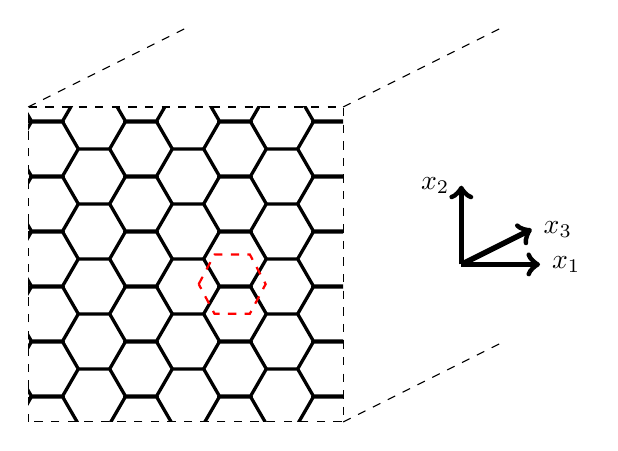
\begin{tikzpicture}

	%x_1,x_2-plane with period cell highlighted
	\draw[pattern=hexagons, dashed] (0,0) rectangle (4,4);	
	%x_3 fibre axes effect
	\draw[dashed] (4,4) -- (6,5);
	\draw[dashed] (4,0) -- (6,1);
	\draw[dashed] (0,4) -- (2,5);
	
	%period cell outline hexagon
	\begin{scope}[scale=1.0, shift={(0.365,0)}]
		\draw[thick, red, dashed] (1.8,1.75) -- (2.0,2.125) -- (2.45,2.125) -- (2.65,1.75) -- (2.45,1.75-3/8) -- (2.0,1.75-3/8) -- cycle;
	\end{scope}
	
	%co-ordinate axes
	\begin{scope}[scale=1.0, shift={(5.5,2)}]
		\draw[->, line width=2.0] (0,0) -- (1,0) node[anchor=west] {$x_1$};
		\draw[->, line width=2.0] (0,0) -- (0,1) node[anchor=east] {$x_2$};
		\draw[->, line width=2.0] (0,0) -- ({2/sqrt(5)}, {1/sqrt(5)}) node[anchor=west] {$x_3$};
	\end{scope}

\end{tikzpicture}

\end{document}